\section{Experimental Results}

\subsection{Generated Images and Data Reading}

Figure~\ref{fig:input-pair} shows the left and right input images actually used by the program.
Figure~\ref{fig:stereo-results} presents, from left to right, the normalized disparity image, the
valid-disparity mask, and the relative-depth visualization. All images are direct references to
program outputs under \codepath{task2/results/}. The images are used to inspect spatial structure;
quantitative conclusions are computed from \codepath{disparity_raw.npy} and
\codepath{depth_proxy.npy}.

\begin{figure}[H]
  \centering
  
\includegraphics[width=0.48\linewidth]{../results/left.png}\hfill
  
\includegraphics[width=0.48\linewidth]{../results/right.png}
  \caption{Official OpenCV aloe stereo input images (left: \texttt{aloeL.jpg}; right: \texttt{aloeR.jpg}).}
  \label{fig:input-pair}
\end{figure}

\begin{figure}[H]
  \centering
  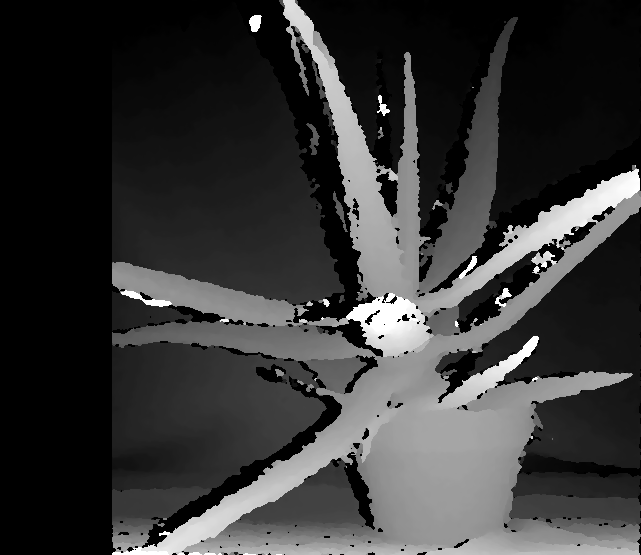
\includegraphics[width=0.31\linewidth]{../results/disparity.png}\hfill
  
\includegraphics[width=0.31\linewidth]{../results/valid_mask.png}\hfill
  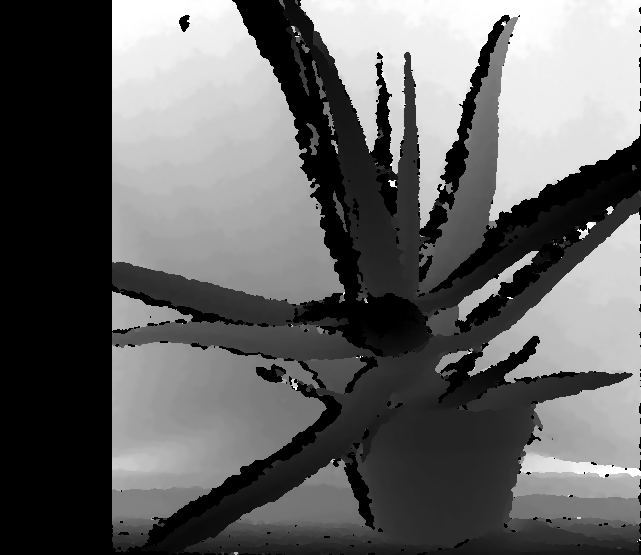
\includegraphics[width=0.31\linewidth]{../results/depth_proxy.png}
  \caption{Program-generated result images, from left to right: normalized disparity, valid-disparity mask, and arbitrary-scale relative depth.}
  \label{fig:stereo-results}
\end{figure}

The normalized PNG files use percentile-based ranges to enhance display contrast, so grayscale
values in a PNG must not be substituted directly into $Z=fB/d$. For example, the raw disparity
at a pixel must be read from \codepath{disparity_raw.npy}; its relative-depth value must be read
from \codepath{depth_proxy.npy}. Both arrays retain the \texttt{NaN} semantics of invalid regions.

\subsection{Results from the Actual Run}

The statistics below are read directly from the floating-point arrays generated by the program.
The arrays have size $555\times641$, for a total of $355755$ pixels. Among the finite disparity
pixels satisfying $d>15$, $261378$ are valid, corresponding to $73.4713\%$ of all pixels.
The actual run results are summarized in Table~\ref{tab:result-statistics}.

\begin{table}[H]
  \centering
  \caption{Measured results from the official OpenCV aloe sample}
  \label{tab:result-statistics}
  \begin{tabular}{ll}
    \toprule
    Metric & Measured value \\
    \midrule
    Original image size & $1282\times1110$ \\
    Matching image size & $641\times555$ \\
    Floating-point array size & $555\times641$ \\
    Total pixels & $355755$ \\
    Valid disparity pixels & $261378$ \\
    Invalid-pixel ratio & $26.5287\%$ \\
    Valid-disparity ratio & $73.4713\%$ \\
    Valid disparity range & $16.000$--$105.875$~px \\
    Relative-depth range & $0.0094451$--$0.0625$ (arbitrary scale) \\
    Formula verification error $\max|z-1/d|$ & $0.0$ \\
    \bottomrule
  \end{tabular}
\end{table}

\subsection{Spatial Distribution of Valid-Matching Coverage}

The global valid ratio only answers what fraction of all processed pixels passes the validity
criterion; it does not indicate whether those pixels are distributed uniformly across the image.
To examine this issue, the $641\times555$ matching image is divided into a $15\times20$ grid, and
each cell is assigned the proportion of pixels that are finite and satisfy $d>15$. The color range
in Fig.~\ref{fig:analysis-coverage} is fixed to 0--100\%, allowing direct comparison between
locations. Blank or light-colored cells indicate that more pixels at those locations failed the
criterion; they do not indicate zero depth.

\begin{figure}[H]
  \centering
  
\includegraphics[width=0.84\linewidth]{figures/analysis_coverage_map.png}
  \caption{Spatial valid-matching coverage. Color denotes the proportion of pixels with finite
  disparity and $d>15$~px in each cell of the $15\times20$ grid. The calculation covers all
  $261378$ valid pixels, giving an overall coverage of $73.4713\%$.}
  \label{fig:analysis-coverage}
\end{figure}

Figure~\ref{fig:analysis-coverage} shows that valid matches are not a uniform region that can be
described only by one global percentage. The coverage varies substantially between grid cells,
indicating that occlusion, insufficient texture, repeated texture, or search-boundary effects may
be spatially concentrated. This figure is therefore a spatial-support diagnostic for the matching
result: it helps locate regions for further inspection, but it is not a disparity-error map and its
color values must not be interpreted as algorithmic accuracy.

\subsection{Numerical Distribution of Valid Disparities}

The $261378$ valid disparity pixels have a range of $16.0000$--$105.8750$~px and a median of
$32.0000$~px. The values of $P_{05}$, $P_{25}$, $P_{75}$, and $P_{95}$ are
$23.7500$, $26.1875$, $53.7500$, and $65.7500$~px, respectively. Figure~\ref{fig:analysis-disparity}
shows the corresponding histogram; the shaded region denotes the interquartile range. The valid
pixels are not concentrated at a single disparity value. Instead, the matching displacement spans
a relatively broad numerical range, which is consistent with surfaces at different front-to-back
positions in the input scene.

\begin{figure}[H]
  \centering
  
\includegraphics[width=0.84\linewidth]{figures/analysis_disparity_distribution.png}
  \caption{Distribution of valid disparities ($n=261378$). Statistics use only finite pixels with
  $d>15$~px; the shaded region denotes $P_{25}$--$P_{75}$, and dashed lines mark $P_{05}$, the
  median, and $P_{95}$. The horizontal axis is measured in pixels.}
  \label{fig:analysis-disparity}
\end{figure}

It is important to emphasize that Fig.~\ref{fig:analysis-disparity} describes the numerical
distribution produced by one StereoSGBM run; it is neither an error distribution nor a confidence
interval. Under $z=1/d$, a larger disparity corresponds to a smaller relative-depth proxy and can
therefore be used to infer relative front-to-back ordering. However, without verified values of
$f$, $B$, and $\mathbf{Q}$, these values cannot be converted to metric depth in meters and the
width of the distribution cannot be interpreted as matching accuracy.

\subsection{Spatial Disparity Heterogeneity and Quadrant Comparison}

The global histogram still cannot answer where the larger or smaller disparities occur. Therefore,
Fig.~\ref{fig:analysis-spatial}(a) displays the median valid disparity in the same $15\times20$
grid, while Fig.~\ref{fig:analysis-spatial}(b) divides the image at its center into upper-left,
upper-right, lower-left, and lower-right quadrants and plots a box plot of all valid disparities in
each region. The corresponding sample counts, regional coverage, medians, and interquartile ranges
are listed in Table~\ref{tab:quadrant-statistics}.

\begin{figure}[H]
  \centering
  
\includegraphics[width=0.99\linewidth]{figures/analysis_spatial_disparity.png}
  \caption{Spatial disparity and quadrant comparison. (a) Color denotes the median valid disparity
  within each grid cell; gray denotes no valid match. (b) Box plots of all valid disparities in the
  four quadrants; the box spans $P_{25}$--$P_{75}$ and the horizontal line marks the median. The
  quadrants are defined only by image coordinates and do not represent semantic object classes.}
  \label{fig:analysis-spatial}
\end{figure}

\begin{table}[H]
  \centering
  \small
  \caption{Valid-disparity statistics for the four image quadrants}
  \label{tab:quadrant-statistics}
  \begin{tabular}{lrrrr}
    \toprule
    Region & Valid samples & Coverage & Median disparity / px & $P_{25}$--$P_{75}$ / px \\
    \midrule
    Upper-left & $51934$ & $58.59\%$ & $28.0000$ & $25.1875$--$30.1875$ \\
    Upper-right & $74778$ & $84.10\%$ & $25.0625$ & $24.0000$--$45.0000$ \\
    Lower-left & $52589$ & $59.12\%$ & $35.8125$ & $32.2500$--$49.1875$ \\
    Lower-right & $82077$ & $91.98\%$ & $53.1250$ & $30.1250$--$56.2500$ \\
    \bottomrule
  \end{tabular}
\end{table}

The four regions differ simultaneously in coverage and median disparity. The lower-right region
has the largest number of valid samples and the highest coverage, with a median disparity of
$53.1250$~px; the upper-right region has a substantially smaller median of $25.0625$~px. Given
the monotonic relationship $z=1/d$, the reported output exhibits observable relative front-to-back
variation across image locations. Because the quadrants are geometric partitions rather than object
segments, these differences cannot be attributed directly to a particular object, nor can they be
used to claim statistical significance or algorithmic superiority.

Figure~\ref{fig:analysis-spatial} also shows within-region dispersion. For example, the boxes and
whiskers in the upper-right and lower-right quadrants span broad ranges, indicating that a single
quadrant contains pixels with different disparities at the same time. Thus, local depth
interpretation should consider spatial position, sample coverage, and the numerical distribution
together; a single high-disparity pixel should not be selected as the ``nearest point.''

\subsection{Quantitative Interpretation of Relative Near--Far Ordering}

After sorting the valid disparities, the lower 0--5\% interval spans $16.000$--$23.750$~px and
has a median relative-depth proxy of $0.043127$. The upper 95--100\% interval spans
$65.750$--$105.875$~px and has a median relative-depth proxy of $0.014172$. The latter is smaller,
as required by the monotonic relationship $1/d$: larger disparity corresponds to a relatively nearer
region.

The disparity and relative-depth images retain the main structures of the leaves, flowerpot, and
background, indicating that StereoSGBM with fixed parameters has produced usable matches. Blank
regions in the valid-disparity mask are not ``zero depth''; they are invalid matches excluded from
the statistics by the program.

\subsection{Result Boundaries}

Invalid regions may arise from occlusion, insufficient texture, repeated texture, or insufficient
search range near the left and right image boundaries. They should not be filled with arbitrary
values merely to make the visualization appear complete. If \texttt{aloeGT.png} is used, it can
only serve as an official disparity reference image; it is not camera calibration or metric-depth
ground truth. Because the current aloe stereo pair has no verified $f$, $B$, or $\mathbf{Q}$, this
experiment cannot report absolute depth in meters or centimeters, nor can it provide a metric-scale
3D point cloud.
